% Options for packages loaded elsewhere
\PassOptionsToPackage{unicode}{hyperref}
\PassOptionsToPackage{hyphens}{url}
%
\documentclass[
]{article}
\usepackage{lmodern}
\usepackage{amssymb,amsmath}
\usepackage{ifxetex,ifluatex}
\ifnum 0\ifxetex 1\fi\ifluatex 1\fi=0 % if pdftex
  \usepackage[T1]{fontenc}
  \usepackage[utf8]{inputenc}
  \usepackage{textcomp} % provide euro and other symbols
\else % if luatex or xetex
  \usepackage{unicode-math}
  \defaultfontfeatures{Scale=MatchLowercase}
  \defaultfontfeatures[\rmfamily]{Ligatures=TeX,Scale=1}
\fi
% Use upquote if available, for straight quotes in verbatim environments
\IfFileExists{upquote.sty}{\usepackage{upquote}}{}
\IfFileExists{microtype.sty}{% use microtype if available
  \usepackage[]{microtype}
  \UseMicrotypeSet[protrusion]{basicmath} % disable protrusion for tt fonts
}{}
\makeatletter
\@ifundefined{KOMAClassName}{% if non-KOMA class
  \IfFileExists{parskip.sty}{%
    \usepackage{parskip}
  }{% else
    \setlength{\parindent}{0pt}
    \setlength{\parskip}{6pt plus 2pt minus 1pt}}
}{% if KOMA class
  \KOMAoptions{parskip=half}}
\makeatother
\usepackage{xcolor}
\IfFileExists{xurl.sty}{\usepackage{xurl}}{} % add URL line breaks if available
\IfFileExists{bookmark.sty}{\usepackage{bookmark}}{\usepackage{hyperref}}
\hypersetup{
  pdftitle={Supplemental Material},
  hidelinks,
  pdfcreator={LaTeX via pandoc}}
\urlstyle{same} % disable monospaced font for URLs
\usepackage[margin=1in]{geometry}
\usepackage{longtable,booktabs}
% Correct order of tables after \paragraph or \subparagraph
\usepackage{etoolbox}
\makeatletter
\patchcmd\longtable{\par}{\if@noskipsec\mbox{}\fi\par}{}{}
\makeatother
% Allow footnotes in longtable head/foot
\IfFileExists{footnotehyper.sty}{\usepackage{footnotehyper}}{\usepackage{footnote}}
\makesavenoteenv{longtable}
\usepackage{graphicx}
\makeatletter
\def\maxwidth{\ifdim\Gin@nat@width>\linewidth\linewidth\else\Gin@nat@width\fi}
\def\maxheight{\ifdim\Gin@nat@height>\textheight\textheight\else\Gin@nat@height\fi}
\makeatother
% Scale images if necessary, so that they will not overflow the page
% margins by default, and it is still possible to overwrite the defaults
% using explicit options in \includegraphics[width, height, ...]{}
\setkeys{Gin}{width=\maxwidth,height=\maxheight,keepaspectratio}
% Set default figure placement to htbp
\makeatletter
\def\fps@figure{htbp}
\makeatother
\setlength{\emergencystretch}{3em} % prevent overfull lines
\providecommand{\tightlist}{%
  \setlength{\itemsep}{0pt}\setlength{\parskip}{0pt}}
\setcounter{secnumdepth}{5}
\usepackage{booktabs}
\usepackage{longtable}
\usepackage{array}
\usepackage{multirow}
\usepackage{wrapfig}
\usepackage{float}
\usepackage{colortbl}
\usepackage{pdflscape}
\usepackage{tabu}
\usepackage{threeparttable}
\usepackage{threeparttablex}
\usepackage[normalem]{ulem}
\usepackage{makecell}
\usepackage{xcolor}

\title{Supplemental Material}
\author{}
\date{\vspace{-2.5em}}

\begin{document}
\maketitle

In Supplemental Figure \ref{fig:boundary}, we show the voxels in the template that had values less than 5 Hounsfield units. We removed these voxels from the final template as they are likely voxels from only a few subjects.

\begin{figure}
\centering
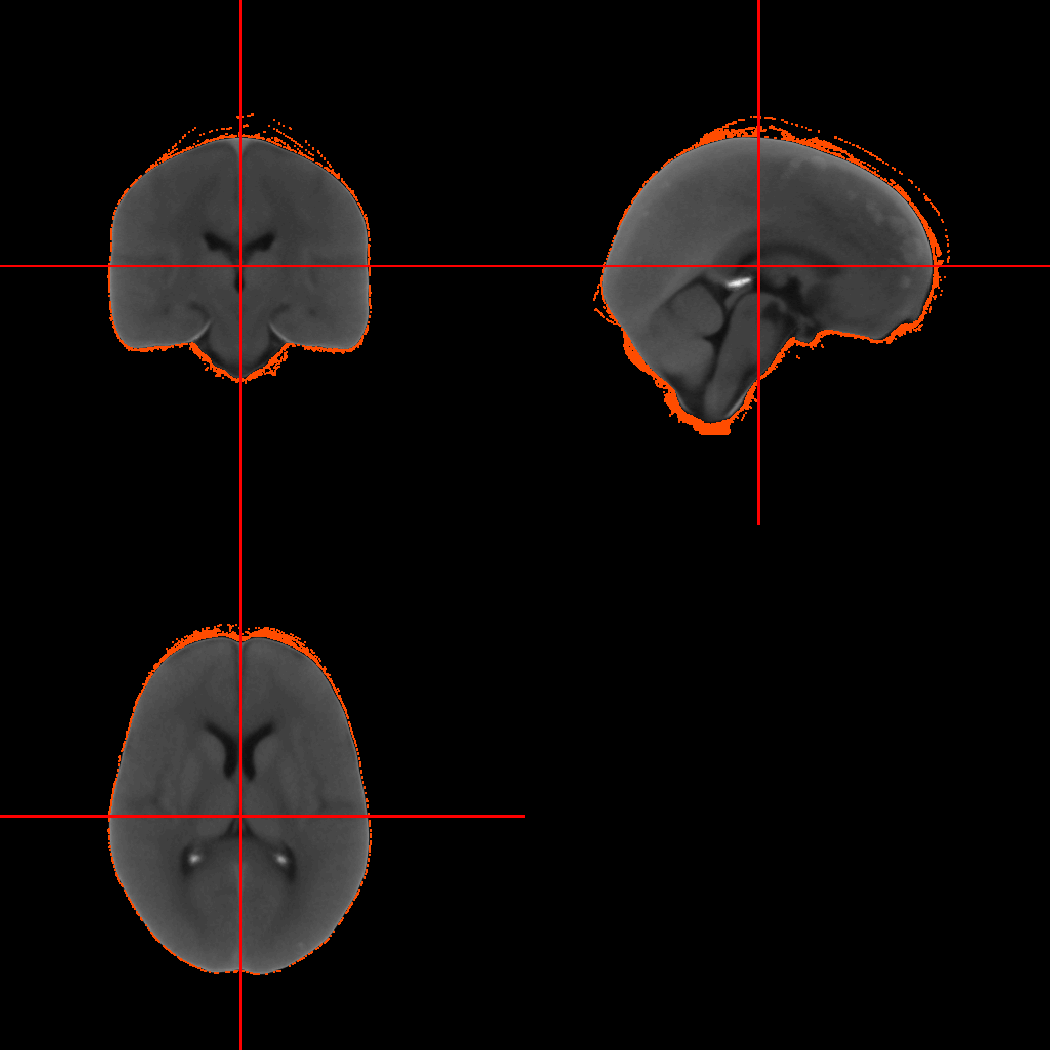
\includegraphics{index_files/figure-latex/sd_image.pdf}
\caption{\label{fig:boundary}Boundary Issues with Low HU Values. Here we present the average image with the mask of voxels that were lower than 5 HU in the template. We excluded these values from the final template.}
\end{figure}

In Supplemental Figure \ref{fig:median} we show the template image, but using the voxel-wise median rather than the mean. We see fewer areas of high intensity, as the median is resistant to large outliers. We do see some brighter areas towards the cortical surface, which may be a byproduct of partial voluming effects with the skull or truly denser areas.

\begin{figure}
\centering
\includegraphics{supplement_files/figure-latex/median-1.pdf}
\caption{\label{fig:median}Median Image. We see fewer areas of high intensity, as the median is resistant to large outliers. We do see some brighter areas towards the cortical surface, which may be a byproduct of partial voluming effects with the skull or truly denser areas.}
\end{figure}

In Supplemental Table \ref{tab:labs} Here we present a set of the labels for the structures in the structural segmentation of the template.

\begin{table}

\caption{\label{tab:labs}Example Structure Labels.  Here we present a set of the labels for the structures in the structural segmentation of the template.}
\centering
\begin{tabular}[t]{r|l}
\hline
index & name\\
\hline
50 & Left Inf Lat Vent\\
\hline
51 & Right Lateral Ventricle\\
\hline
52 & Left Lateral Ventricle\\
\hline
53 & Right Lesion\\
\hline
54 & Left Lesion\\
\hline
55 & Right Pallidum\\
\hline
56 & Left Pallidum\\
\hline
57 & Right Putamen\\
\hline
58 & Left Putamen\\
\hline
59 & Right Thalamus Proper\\
\hline
60 & Left Thalamus Proper\\
\hline
61 & Right Ventral DC\\
\hline
62 & Left Ventral DC\\
\hline
63 & Right vessel\\
\hline
64 & Left vessel\\
\hline
65 & Left Insula\\
\hline
66 & Right Insula\\
\hline
67 & Left Operculum\\
\hline
68 & Right Operculum\\
\hline
69 & Optic Chiasm\\
\hline
70 & Basal Forebrain\\
\hline
\end{tabular}
\end{table}

\end{document}
